\apendice{Especificación de diseño}

\section{Introducción}
En este apartado lo que se pretende es indagar en la estructura que se ha seguido para el desarrollo del estudio desde la perspectiva del diseño, tanto de los datos como procedimental y arquitectónico.

\section{Diseño de datos}
Una vez los datos son procesados por Logstash y previo a su exposición en un \textit{dashboard} de Kibana, estos son almacenados en ElasticSearch en forma de indices que se pueden o generar en el momento de carga, o generar previamente por línea de comando en la terminal \textit{Dev Tools} de Elastic. Esta sección se va a centrar en analizar como se gestionan y almacenan esos datos, y de que forma son estructurados en Elastic.

\paragraph{}

Un índice en ElasticSearch consiste en un almacen de documentos que contienen campos en forma de claves clave-valor que almacenan los datos \cite{indices}. En este estudio se han analizado cinco escenarios, conteniendo toda la información de cada escenario en índices aislados de manera que se siga una estructrua ordenada.

\paragraph{}
\paragraph{}
\paragraph{}


Para el primero de los escenarios, en el cuál se realiza la ingesta de un archivo de tipo CSV directamente desde Elastic, el índice que se generó recibe el nombre de \textit{titanic}, puesto que el archivo original tiene este nombre \ref{fig:indice1}. Contiene 891 documentos equivalente a las 891 líneas de registro que posee el archivo original, y el mapeo de este índice está estructurado de la siguiente forma:

\{ "mappings": \{ "\_meta": \{ "created\_by": "file-data-visualizer" \}, 
"properties": \{ "\textbf{Age}": \{ "type": "double" \}, "\textbf{Cabin}": \{ "type": "keyword" \}, "\textbf{Embarked}": \{ "type": "keyword" \}, "\textbf{Fare}": \{ "type": "double" \}, "\textbf{Name}": \{ "type": "text" \}, "\textbf{Parch}": \{ "type": "long" \}, "\textbf{PassengerId}": \{ "type": "long" \}, "\textbf{Pclass}": \{ "type": "long" \}, "\textbf{Sex}": \{ "type": "keyword" \}, "\textbf{SibSp}": \{ "type": "long" \}, "\textbf{Survived}": \{ "type": "long" \}, "\textbf{Ticket}": \{ "type": "keyword" \} \} \} \} 

Incluyendo en el apartado \textit{properties} los datos del nombre y el tipo de cada campo del archivo, de manera que una vez los datos seán cargados, Elastic comprenda de que tipo es cada valor cargado.

\begin{figure}
    \centering
    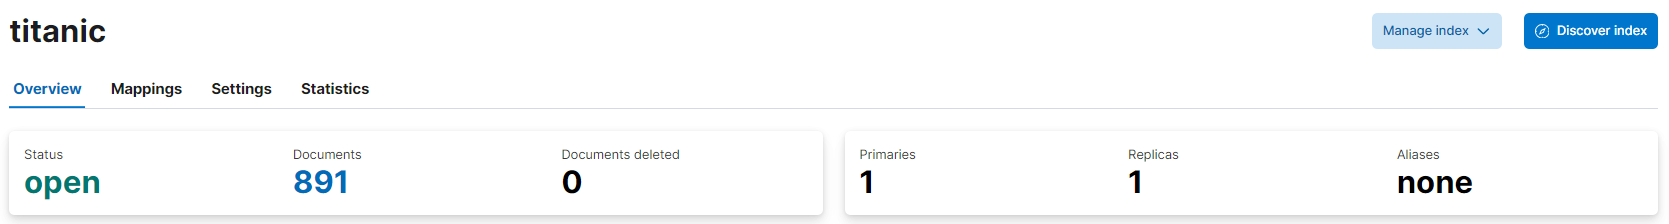
\includegraphics[width=1\linewidth]{img/titanic1.png}
    \caption{Descripción del índice del primer escenario.}
    \label{fig:indice1}
\end{figure}

En el siguiente escenario, en el cuál se realiza la ingesta de archivo pasando por Logstash donde se le aplican una serie de modificaciones antes de llegar a Elastic, el índice creado recibe el nombre de \textit{casas}, puesto que el archivo contiene información de distintas vivendas \ref{fig:indice2}. Posee 80 documentos equivalente a las 80 casas en venta que tiene la inmobiliaria y el mapeo tiene la siguiente estructura:

\{ "mappings": \{ "properties": \{ "@\textbf{timestamp}": \{ "type": "date" \}, "\textbf{barrio}": \{ "type": "keyword" \}, "\textbf{categoria}": \{ "type": "keyword" \}, "\textbf{ciudad}": \{ "type": "keyword" \}, "\textbf{metros\_cuadrados}": \{ "type": "float" \}, "\textbf{num\_casa}": \{ "type": "integer" \}, "\textbf{num\_habitaciones}": \{ "type": "integer" \}, "\textbf{precio}": \{ "type": "float" \} \} \} \}

Incluyendo en el apartado \textit{properties} los datos del nombre y el tipo de cada campo del archivo, de manera que una vez los datos seán cargados, Elastic comprenda de que tipo es cada valor cargado.

\begin{figure}
    \centering
    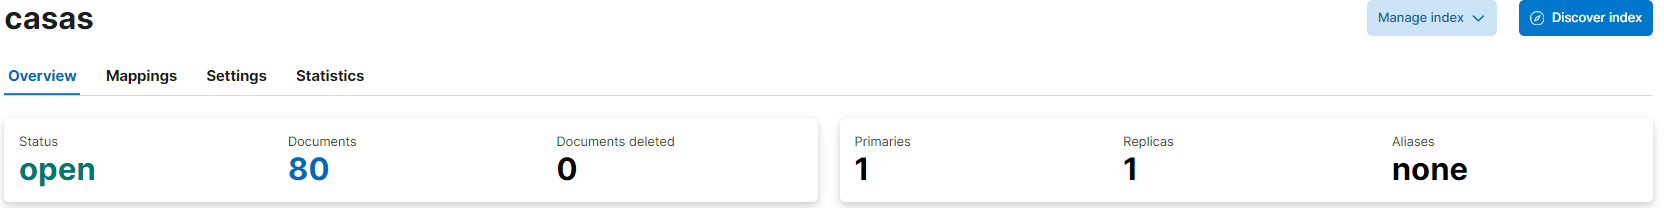
\includegraphics[width=1\linewidth]{img/indice2.png}
    \caption{Descripción del índice del segundo escenario.}
    \label{fig:indice2}
\end{figure}

En los siguientes dos escenarios la dificultad se volvió mayor puesto que se trabajó con streams de datos, por lo que los índices de estos dos escenarios son más complejos que los anteriores y ocupan un mayor tamaño. En el caso del tercer escenario, el índice recibe el nombre de \textit{websockets-data} \ref{fig:indice3}, y tiene un tamaño cambiante en función del tiempo que esté expuesto a la carga de datos por parte del script del WebSocket. Tiene el siguiente mapeo puesto que los datos que llegan son tal cuál los que se mandan por el WebSocket:

\{ "mappings": \{ "properties": \{ "@\textbf{timestamp}": \{ "type": "date" \}, "data": \{ "properties": \{ "\textbf{c}": \{ "type": "text", "fields": \{ "keyword": \{ "type": "keyword", "ignore\_above": 256 \} \} \}, "\textbf{p}": \{ "type": "float" \}, "\textbf{s}": \{ "type": "text", "fields": \{ "keyword": \{ "type": "keyword", "ignore\_above": 256 \} \} \}, "\textbf{t}": \{ "type": "long" \}, "\textbf{v}": \{ "type": "float" \} \} \}, "type": \{ "type": "text", "fields": \{ "keyword": \{ "type": "keyword", "ignore\_above": 256 \} \} \} \} \} \} 

En el cuál llegan cinco campos con nombres de letras los cuáles serán ignorados si su longitud máxima excede los 256 caracteres.

\begin{figure}
    \centering
    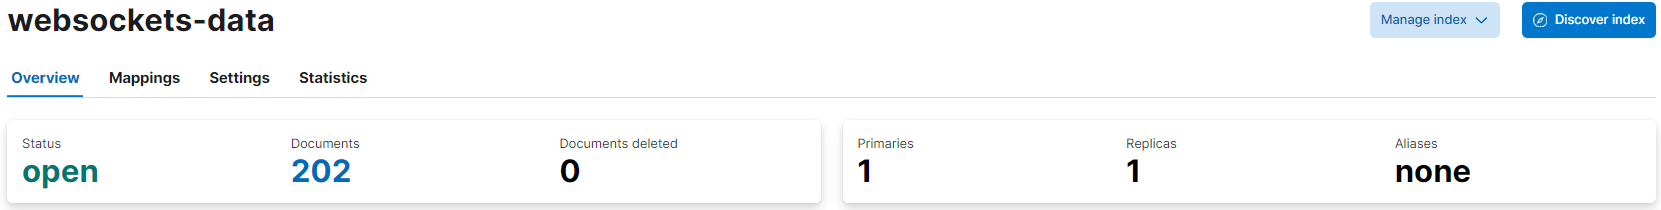
\includegraphics[width=1\linewidth]{img/indice3.png}
    \caption{Descripción del índice del tercer escenario.}
    \label{fig:indice3}
\end{figure}

En el cuarto escenario la descripción del índice es la misma, salvando que en este caso recibe el nombre de \textit{test-data-stream} \ref{fig:indice4}. El mapeo del contenido tendrá la siguiente forma una vez los datos: 

\{ "mappings": \{ "dynamic": "true", "dynamic\_date\_formats": [ "strict\_date\_optional\_time", "yyyy/MM/dd HH:mm:ss Z||yyyy/MM/dd Z"], "dynamic\_templates": [], "date\_detection": true, "numeric\_detection": true, "properties": \{ "@\textbf{timestamp}": \{ "type": "date", "format": "strict\_date\_optional\_time" \}, "@\textbf{version}": \{ "type": "long" \}, "data": \{ "properties": \{ "\textbf{LastPrice}": \{ "type": "float" \}, "\textbf{Symbol}": \{ "type": "text", "fields": \{ "keyword": \{ "type": "keyword", "ignore\_above": 256 \}\}\}, "\textbf{Timestamp}": \{ "type": "long" \}, "\textbf{TotalPrice}": \{ "type": "float" \}, "\textbf{Volume}": \{ "type": "float" \}\}\}

Como se puede observar las variables que antes eran letras ahora tienen un nombre que describe la información que contiene, así como la inclusión de nuevos campos como son la versión y el precio total.

\begin{figure}
    \centering
    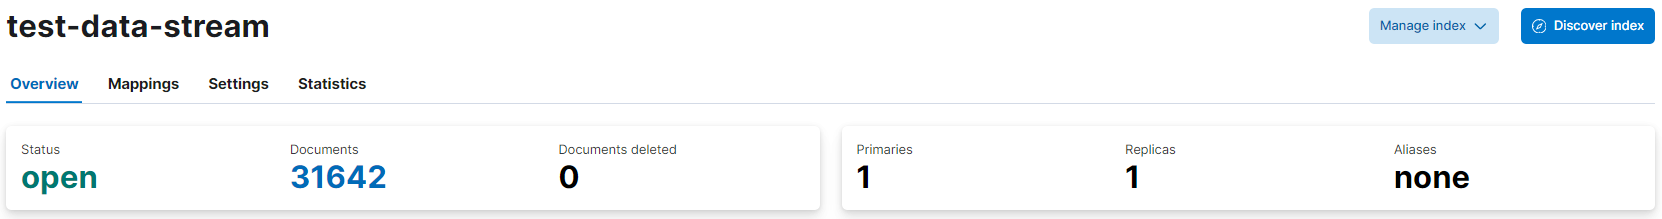
\includegraphics[width=1\linewidth]{img/indice4.png}
    \caption{Descripción del índice del cuarto escenario.}
    \label{fig:indice4}
\end{figure}

En el quinto y último escenario, en el cuál se ingesta un streaming de datos en vivo aplicando MapReduce en Logstash antes de llegar a Elastic, el índice que se ha creado recibe el nombre de \textit{transactions aggregate} \ref{fig:indice5}, y contiene tan solo 3 filas por los 3 métodos de pago existentes, que es la variable que se ha tomado como referencia para hacer el MapReduce. El mapeo de los campos cargados tiene la siguiente estructura:

\{ "mappings": \{ "properties": \{ 
"@\textbf{timestamp}": \{ "type": "date" \}, 
"@\textbf{version}": \{ "type": "text", "fields": \{ "keyword": \{ "type": "keyword", "ignore\_above": 256 \} \} \}, 
"\textbf{amount}": \{ "type": "float" \}, 
"\textbf{city}": \{ "type": "text", "fields": \{ "keyword": \{ "type": "keyword", "ignore\_above": 256 \} \} \}, 
"\textbf{country}": \{ "type": "text", "fields": \{ "keyword": \{ "type": "keyword", "ignore\_above": 256 \} \} \}, 
"\textbf{customer\_id}": \{ "type": "text", "fields": \{ "keyword": \{ "type": "keyword", "ignore\_above": 256 \} \} \}, "event": \{ "properties": \{ "original": \{ "type": "text", "fields": \{ "keyword": \{ "type": "keyword", "ignore\_above": 256 \} \} \} \} \}, "host": \{ "properties": \{ "name": \{ "type": "text", "fields": \{ "keyword": \{ "type": "keyword", "ignore\_above": 256 \} \} \} \} \}, "log": \{ "properties": \{ "file": \{ "properties": \{ "path": \{ "type": "text", "fields": \{ "keyword": \{ "type": "keyword", "ignore\_above": 256 \} \} \} \} \} \} \}, 
"\textbf{payment\_method}": \{ "type": "text", "fields": \{ "keyword": \{ "type": "keyword", "ignore\_above": 256 \} \} \}, 
"\textbf{product\_category}": \{ "type": "text", "fields": \{ "keyword": \{ "type": "keyword", "ignore\_above": 256 \} \} \}, 
"\textbf{timestamp}": \{ "type": "date" \}, 
"\textbf{total\_amount}": \{ "type": "float" \}, 
"\textbf{transaction\_id}": \{ "type": "text", "fields": \{ "keyword": \{ "type": "keyword", "ignore\_above": 256 \} \} \} \} \} \} 

Almacenando todas los campos presentes en el streaming de datos de manera que se pueda completar los 3 documentos con información interesante recopilada de los datos.

\begin{figure}
    \centering
    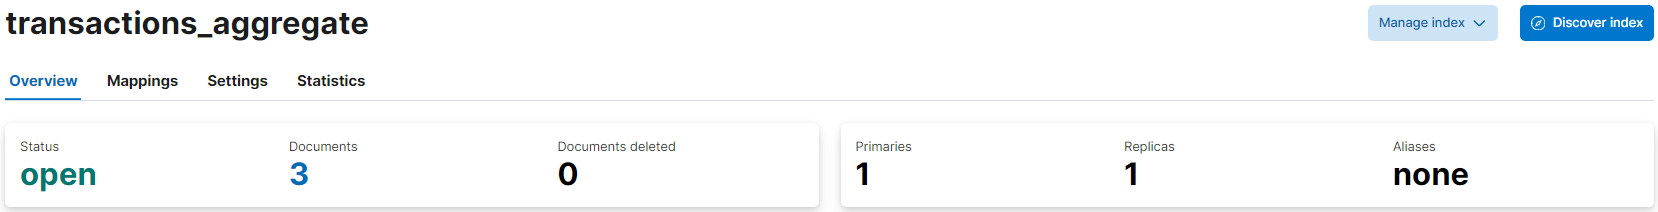
\includegraphics[width=1\linewidth]{img/indice5.png}
    \caption{Descripción del índice del quinto escenario.}
    \label{fig:indice5}
\end{figure}

\section{Diseño procedimental}

En esta sección se van a abordar los procesos seguidos para ejecutar el procesamiento de los datos en cada uno de los cinco escenarios con las herramientas ELK.

El caso del primer escenario es el más sencillo de todos, puesto que la ingesta del archivo de tipo CSV se hace directamente desde el menú interactivo de Elastic, en la opción \textit{upload file} \ref{fig:ingesta1}, donde mediante un mecanismo de \textit{drag and drop} Elastic permite la importación de archivos CSV, TSV, o JSON entre otros. 

\begin{figure}
    \centering
    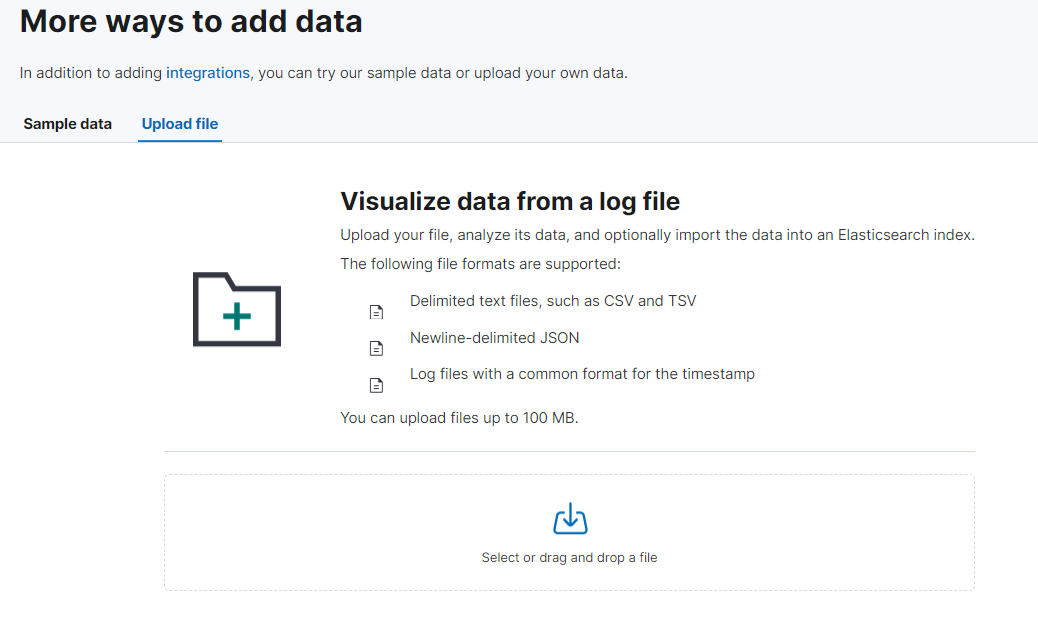
\includegraphics[width=1\linewidth]{img/ingesta1.png}
    \caption{Menú de importación de archivos de Elastic.}
    \label{fig:ingesta1}
\end{figure}

En el segundo escenario, Logstash está de por medio entre la fuente de datos y ElasticSearch, por lo que es ahí donde ocurre todo el procesamiento de los datos. Primero, indicando en al apartado \textit{input} del archivo de configuración para este escenario desde donde se van a ingestar los datos en Logstash \ref{fig:ingesta2}, en este caso se introduce la ruta \textit{path} hacia el archivo casas.log, del cuál se extrae la información, se indica la posición desde donde se quiere empezar a leer, si partimos de una base de datos guardada y la codificación del archivo.

\begin{figure}
    \centering
    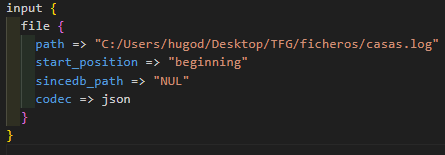
\includegraphics[width=1\linewidth]{img/ingesta2.png}
    \caption{Apartado de ingesta del segundo escenario.}
    \label{fig:ingesta2}
\end{figure}

Una vez el archivo es cargado en Logstash, ya se le pueden realizar todas las transformaciones y modificaciones oportunas en el apartado \textit{filter}. Tras esto, los datos procesados deben ir al destino que se indique en el apartado \textit{output} \ref{fig:ingesta22}, en este caso primero se mandaran a Elastic indicando la ruta del puerto local, el nombre del índice donde se alojaran y que hay que crear, así como el usuario y contraseña de Elastic en caso de que fueran necesarios. Tambien se indica que los datos deben ser mostrados por terminal para comprobar que el proceso a sido satisfactorio.

\begin{figure}
    \centering
    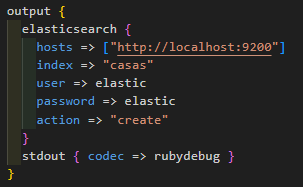
\includegraphics[width=1\linewidth]{img/ingesta2-2.png}
    \caption{Apartado de exportación de los datos tratados.}
    \label{fig:ingesta22}
\end{figure}

Para el tercer escenario, en el que se trabaja con un stream de datos directamente sobre Elastic, todo el proceso de ingesta se realiza en el script escrito en Python del mismo. Primeramente se indica en la variable \textit{client} cuál es el puerto local destino de los datos, y en la función \textit{message} se almacenará la fecha y los datos en el índice \textit{websockets data} \ref{fig:ingesta31}. En la parte final se encuentra la suscripción a diferentes divisas criptográficas, así como el token para utilizar la API de Finnhub, la cuál estará mandando datos hasta que se detenga el script \ref{fig:ingesta32}.

\begin{figure}
    \centering
    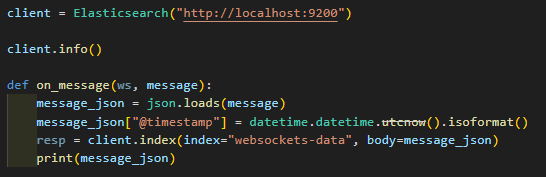
\includegraphics[width=1\linewidth]{img/ingesta31.png}
    \caption{Sección del script indicando datos de la ingesta del tercer escenario.}
    \label{fig:ingesta31}
\end{figure}
\begin{figure}
    \centering
    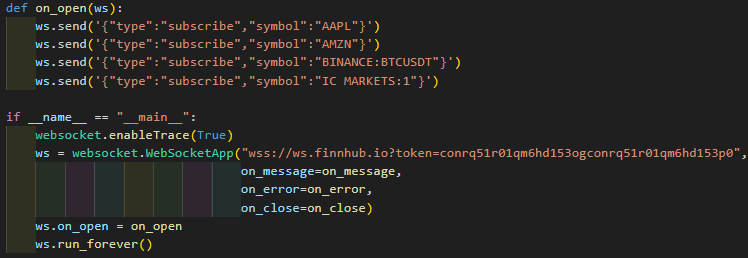
\includegraphics[width=1\linewidth]{img/ingesta32.png}
    \caption{Sección del script indicando más datos de la ingesta del tercer escenario.}
    \label{fig:ingesta32}
\end{figure}

El cuarto escenario, al ser una modificación del tercero, tendrá una estructura del procedimiento de ingesta de datos similar. La primera diferencia será en la parte inicial del script \ref{fig:ingesta41}, donde se añadirá una nueva función que renombre los campos recibidos de manera que sea más entendible la información que proporcionan. También cambia la ruta del destino de los datos, puesto que a través del protocolo HTTP los datos serán enviados al puerto 8080 donde Logstash estará escuchando a la espera de información.

\begin{figure}
    \centering
    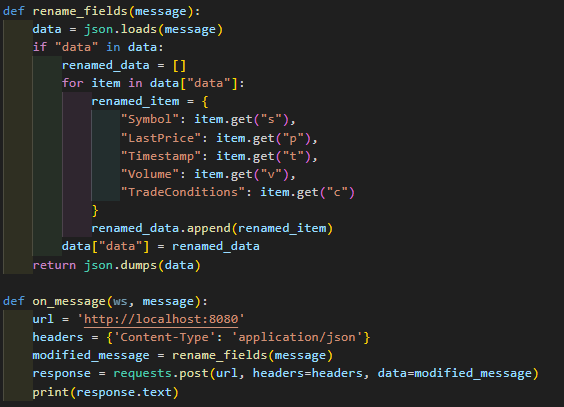
\includegraphics[width=1\linewidth]{img/ingesta41.png}
    \caption{Primera parte de la ingesta del cuarto escenario.}
    \label{fig:ingesta41}
\end{figure}

\paragraph{}
\paragraph{}
\paragraph{}
\paragraph{}
\paragraph{}
\paragraph{}
\paragraph{}
\paragraph{}
\paragraph{}


El resto del script tiene una estructura idéntica al del tercer escenario. Una vez los datos son mandados al puerto 8080, Logstash tendrá especificado en el apartado \textit{input} que tiene que estar escuchando de ese puerto a través del protocolo HTTP \ref{fig:ingesta42}. Una vez cargados en tiempo real, la información es procesada con las transformaciones del apartado \textit{filter} y mandadas a Elastic al índice \textit{test data stream} como se especifica en el apartado \textit{output} del archivo de configuración \ref{fig:ingesta43}.  

\begin{figure}
    \centering
    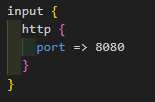
\includegraphics[width=1\linewidth]{img/ingesta42.png}
    \caption{Segunda parte de la ingesta de datos del cuarto escenario.}
    \label{fig:ingesta42}
\end{figure}

\begin{figure}
    \centering
    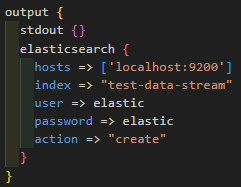
\includegraphics[width=1\linewidth]{img/ingesta43.png}
    \caption{Úiltima parte del proceso de ingesta del cuarto escenario.}
    \label{fig:ingesta43}
\end{figure}

Para el último escenario en el que aplicamos MapReduce a una transmisión de datos en vivo, el proceso de ingesta tiene varias partes. La primera será el script que genera estos datos en vivo \ref{fig:ingesta51}, en el cuál se especifica la ruta del archivo donde se almacenarán los registros, así como los campos sobre los que se van a ir generando valores aleatorios en función de los indicados. 

\begin{figure}
    \centering
    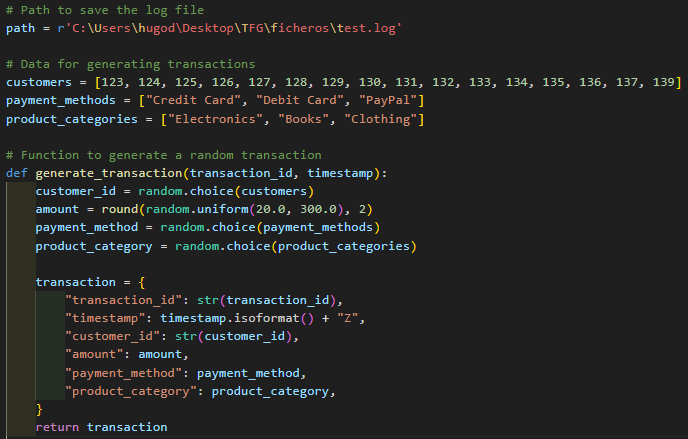
\includegraphics[width=1\linewidth]{img/ingesta51.png}
    \caption{Script de generación de datos del quinto escenario.}
    \label{fig:ingesta51}
\end{figure}

\paragraph{}
\paragraph{}

Una vez se ejecuta el script los registros se van escribiendo del archivo del cuál Logstash está informado para poder realizar el MapReduce \ref{fig:ingesta52}. Una vez se detiene la carga de datos a Logstash por parte del script, este mandará la información procesada a Elastic dirigiéndose hacia el índice indicado \ref{fig:ingesta53}.

\begin{figure}
    \centering
    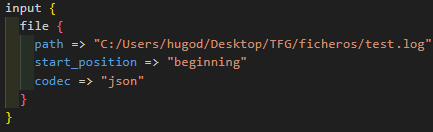
\includegraphics[width=1\linewidth]{img/ingesta52.png}
    \caption{Ingesta de datos del script a Logstash en el quinto escenario.}
    \label{fig:ingesta52}
\end{figure}

\begin{figure}
    \centering
    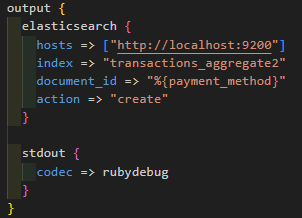
\includegraphics[width=1\linewidth]{img/ingesta53.png}
    \caption{Destino final para los datos del quinto escenario.}
    \label{fig:ingesta53}
\end{figure}

\paragraph{}
\paragraph{}
\paragraph{}
\paragraph{}
\paragraph{}
\paragraph{}
\paragraph{}
\paragraph{}
\paragraph{}
\paragraph{}
\paragraph{}
\paragraph{}
\paragraph{}


\section{Diseño arquitectónico}

El estudio se ha estrcutrado en un sistema ELK, compuesto por ElasticSearch, Logstash y Kibana, así como de una fuente desde donde se ingestan los datos. Estos cuatro elementos conforman la arquitecturá básica del proyecto \ref{fig:elk}.

La fuente de ingesta de datos ha ido variando en función de la situación que se quería mostrar en cada escenario. Siendo un archivo de tipo CSV en el primero, un archivo de tipo .log en el segundo y streamings de datos en los demás. Lo que permance inamovible son los otros tres componentes del proyecto, ElasticSearch, siendo empleado en todos los escenarios como base de almacenamiento y búsqueda de los datos, Logstash, como intermediario entre Elastic y la fuente de datos para procesar y transformar la información de estos antes de ser cargada, y por último pero no menos importante, Kibana, cumpliendo el papel de expositor para la información procesada y cargada previamente por los otros componentes.

\begin{figure}
    \centering
    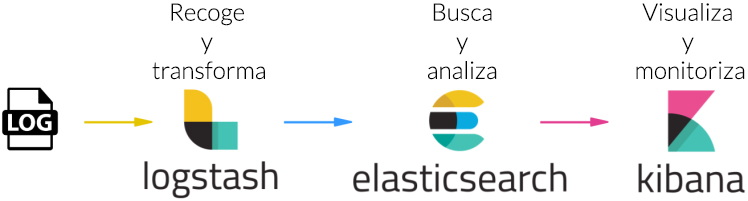
\includegraphics[width=1\linewidth]{img/elk.jpg}
    \caption{Arquitectura del sistema ELK.}
    \label{fig:elk}
\end{figure}
